\documentclass[twoside]{book}

% Packages required by doxygen
\usepackage{fixltx2e}
\usepackage{calc}
\usepackage{doxygen}
\usepackage[export]{adjustbox} % also loads graphicx
\usepackage{graphicx}
\usepackage[utf8]{inputenc}
\usepackage{makeidx}
\usepackage{multicol}
\usepackage{multirow}
\PassOptionsToPackage{warn}{textcomp}
\usepackage{textcomp}
\usepackage[nointegrals]{wasysym}
\usepackage[table]{xcolor}

% NLS support packages
\usepackage[spanish]{babel}
% Font selection
\usepackage[T1]{fontenc}
\usepackage[scaled=.90]{helvet}
\usepackage{courier}
\usepackage{amssymb}
\usepackage{sectsty}
\renewcommand{\familydefault}{\sfdefault}
\allsectionsfont{%
  \fontseries{bc}\selectfont%
  \color{darkgray}%
}
\renewcommand{\DoxyLabelFont}{%
  \fontseries{bc}\selectfont%
  \color{darkgray}%
}
\newcommand{\+}{\discretionary{\mbox{\scriptsize$\hookleftarrow$}}{}{}}

% Page & text layout
\usepackage{geometry}
\geometry{%
  a4paper,%
  top=2.5cm,%
  bottom=2.5cm,%
  left=2.5cm,%
  right=2.5cm%
}
\tolerance=750
\hfuzz=15pt
\hbadness=750
\setlength{\emergencystretch}{15pt}
\setlength{\parindent}{0cm}
\setlength{\parskip}{3ex plus 2ex minus 2ex}
\makeatletter
\renewcommand{\paragraph}{%
  \@startsection{paragraph}{4}{0ex}{-1.0ex}{1.0ex}{%
    \normalfont\normalsize\bfseries\SS@parafont%
  }%
}
\renewcommand{\subparagraph}{%
  \@startsection{subparagraph}{5}{0ex}{-1.0ex}{1.0ex}{%
    \normalfont\normalsize\bfseries\SS@subparafont%
  }%
}
\makeatother

% Headers & footers
\usepackage{fancyhdr}
\pagestyle{fancyplain}
\fancyhead[LE]{\fancyplain{}{\bfseries\thepage}}
\fancyhead[CE]{\fancyplain{}{}}
\fancyhead[RE]{\fancyplain{}{\bfseries\leftmark}}
\fancyhead[LO]{\fancyplain{}{\bfseries\rightmark}}
\fancyhead[CO]{\fancyplain{}{}}
\fancyhead[RO]{\fancyplain{}{\bfseries\thepage}}
\fancyfoot[LE]{\fancyplain{}{}}
\fancyfoot[CE]{\fancyplain{}{}}
\fancyfoot[RE]{\fancyplain{}{\bfseries\scriptsize Generado por Doxygen }}
\fancyfoot[LO]{\fancyplain{}{\bfseries\scriptsize Generado por Doxygen }}
\fancyfoot[CO]{\fancyplain{}{}}
\fancyfoot[RO]{\fancyplain{}{}}
\renewcommand{\footrulewidth}{0.4pt}
\renewcommand{\chaptermark}[1]{%
  \markboth{#1}{}%
}
\renewcommand{\sectionmark}[1]{%
  \markright{\thesection\ #1}%
}

% Indices & bibliography
\usepackage{natbib}
\usepackage[titles]{tocloft}
\setcounter{tocdepth}{3}
\setcounter{secnumdepth}{5}
\makeindex

% Hyperlinks (required, but should be loaded last)
\usepackage{ifpdf}
\ifpdf
  \usepackage[pdftex,pagebackref=true]{hyperref}
\else
  \usepackage[ps2pdf,pagebackref=true]{hyperref}
\fi
\hypersetup{%
  colorlinks=true,%
  linkcolor=blue,%
  citecolor=blue,%
  unicode%
}

% Custom commands
\newcommand{\clearemptydoublepage}{%
  \newpage{\pagestyle{empty}\cleardoublepage}%
}

\usepackage{caption}
\captionsetup{labelsep=space,justification=centering,font={bf},singlelinecheck=off,skip=4pt,position=top}

%===== C O N T E N T S =====

\begin{document}

% Titlepage & ToC
\hypersetup{pageanchor=false,
             bookmarksnumbered=true,
             pdfencoding=unicode
            }
\pagenumbering{roman}
\begin{titlepage}
\vspace*{7cm}
\begin{center}%
{\Large Gestión de intervalos \\[1ex]\large 0 }\\
\vspace*{1cm}
{\large Generado por Doxygen 1.8.11}\\
\end{center}
\end{titlepage}
\clearemptydoublepage
\tableofcontents
\clearemptydoublepage
\pagenumbering{arabic}
\hypersetup{pageanchor=true}

%--- Begin generated contents ---
\chapter{Índice de clases}
\section{Lista de clases}
Lista de las clases, estructuras, uniones e interfaces con una breve descripción\+:\begin{DoxyCompactList}
\item\contentsline{section}{\hyperlink{classCirculo}{Circulo} }{\pageref{classCirculo}}{}
\item\contentsline{section}{\hyperlink{classPunto}{Punto} \\*Clase \hyperlink{classPunto}{Punto} }{\pageref{classPunto}}{}
\end{DoxyCompactList}

\chapter{Indice de archivos}
\section{Lista de archivos}
Lista de todos los archivos documentados y con descripciones breves\+:\begin{DoxyCompactList}
\item\contentsline{section}{\hyperlink{intervalo_8cpp}{intervalo.\+cpp} }{\pageref{intervalo_8cpp}}{}
\end{DoxyCompactList}

\chapter{Documentación de las clases}
\hypertarget{classIntervalo}{}\section{Referencia de la Clase Intervalo}
\label{classIntervalo}\index{Intervalo@{Intervalo}}
\subsection*{Métodos públicos}
\begin{DoxyCompactItemize}
\item 
\hyperlink{classIntervalo_a9b5b23dda7ee26b444898457959cb03d}{Intervalo} ()\hypertarget{classIntervalo_a9b5b23dda7ee26b444898457959cb03d}{}\label{classIntervalo_a9b5b23dda7ee26b444898457959cb03d}

\begin{DoxyCompactList}\small\item\em Crea un intervalo vacio. \end{DoxyCompactList}\item 
\hyperlink{classIntervalo_a321e56ef7e1f4a774bd64cc2609156f4}{Intervalo} (double cota\+Inferior, double cota\+Superior)
\begin{DoxyCompactList}\small\item\em Crea un \hyperlink{classIntervalo}{Intervalo} cerrado. \end{DoxyCompactList}\item 
\hyperlink{classIntervalo_af70d523399465f51862977a303656c72}{Intervalo} (double cota\+Inferior, double cota\+Superior, bool cerrado\+Inferior, bool cerrado\+Superior)
\begin{DoxyCompactList}\small\item\em Crea un intervalo cualquiera. \end{DoxyCompactList}\item 
double \hyperlink{classIntervalo_af8170b68c6d6a63192db6685b90f782f}{get\+Cota\+Inf} () const 
\begin{DoxyCompactList}\small\item\em Devuelve la cota inferior del intervalo. \end{DoxyCompactList}\item 
double \hyperlink{classIntervalo_a7f8ff94ce16f90a81a3c55f36044893b}{get\+Cota\+Sup} () const 
\begin{DoxyCompactList}\small\item\em Devuelve la cota superior del intervalo. \end{DoxyCompactList}\item 
bool \hyperlink{classIntervalo_a6737cfbda201a3a6e11a716d2568d322}{es\+Cerrado\+Inf} () const 
\begin{DoxyCompactList}\small\item\em Consulta si el intervalo es cerrado en su cota inferior. \end{DoxyCompactList}\item 
bool \hyperlink{classIntervalo_ad0c5573ee88ffbfda8f78454b78d91a6}{es\+Cerrado\+Sup} () const 
\begin{DoxyCompactList}\small\item\em Consulta si el intervalo es cerrado en su cota superior. \end{DoxyCompactList}\item 
bool \hyperlink{classIntervalo_ab53adad27de8ec98cf8f4280bd3a7df9}{es\+Vacio} () const 
\begin{DoxyCompactList}\small\item\em Consulta si el intervalo almacenado es vacío o no. \end{DoxyCompactList}\item 
bool \hyperlink{classIntervalo_af55ac0bb47855ef909402e2ec76cda5b}{esta\+Dentro} (double n) const 
\begin{DoxyCompactList}\small\item\em Consulta si un determinado valor está dentro del intervalo. \end{DoxyCompactList}\end{DoxyCompactItemize}


\subsection{Descripción detallada}


Definición en la línea 12 del archivo intervalo.\+cpp.



\subsection{Documentación del constructor y destructor}
\index{Intervalo@{Intervalo}!Intervalo@{Intervalo}}
\index{Intervalo@{Intervalo}!Intervalo@{Intervalo}}
\subsubsection[{\texorpdfstring{Intervalo(double cota\+Inferior, double cota\+Superior)}{Intervalo(double cotaInferior, double cotaSuperior)}}]{\setlength{\rightskip}{0pt plus 5cm}Intervalo\+::\+Intervalo (
\begin{DoxyParamCaption}
\item[{double}]{cota\+Inferior, }
\item[{double}]{cota\+Superior}
\end{DoxyParamCaption}
)}\hypertarget{classIntervalo_a321e56ef7e1f4a774bd64cc2609156f4}{}\label{classIntervalo_a321e56ef7e1f4a774bd64cc2609156f4}


Crea un \hyperlink{classIntervalo}{Intervalo} cerrado. 


\begin{DoxyParams}{Parámetros}
{\em cota\+Inferior} & \\
\hline
{\em cota\+Superior} & \\
\hline
\end{DoxyParams}
\begin{DoxyPrecond}{Precondición}
El intervalo es válido 
\end{DoxyPrecond}


Definición en la línea 98 del archivo intervalo.\+cpp.


\begin{DoxyCode}
98                                            \{
99     assert (validar(cinf,csup, \textcolor{keyword}{true}, \textcolor{keyword}{true}));
100     cotaInf = cinf;
101     cotaSup = csup;
102     cerradoInf = \textcolor{keyword}{true};
103     cerradoSup = \textcolor{keyword}{true};
104 \}
\end{DoxyCode}


Gráfico de llamadas para esta función\+:\nopagebreak
\begin{figure}[H]
\begin{center}
\leavevmode
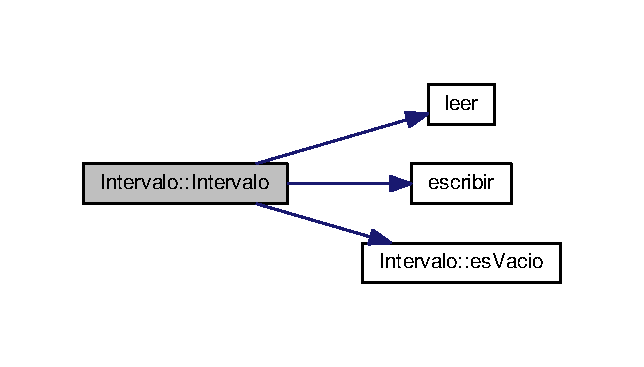
\includegraphics[width=309pt]{classIntervalo_a321e56ef7e1f4a774bd64cc2609156f4_cgraph}
\end{center}
\end{figure}


\index{Intervalo@{Intervalo}!Intervalo@{Intervalo}}
\index{Intervalo@{Intervalo}!Intervalo@{Intervalo}}
\subsubsection[{\texorpdfstring{Intervalo(double cota\+Inferior, double cota\+Superior, bool cerrado\+Inferior, bool cerrado\+Superior)}{Intervalo(double cotaInferior, double cotaSuperior, bool cerradoInferior, bool cerradoSuperior)}}]{\setlength{\rightskip}{0pt plus 5cm}Intervalo\+::\+Intervalo (
\begin{DoxyParamCaption}
\item[{double}]{cota\+Inferior, }
\item[{double}]{cota\+Superior, }
\item[{bool}]{cerrado\+Inferior, }
\item[{bool}]{cerrado\+Superior}
\end{DoxyParamCaption}
)}\hypertarget{classIntervalo_af70d523399465f51862977a303656c72}{}\label{classIntervalo_af70d523399465f51862977a303656c72}


Crea un intervalo cualquiera. 


\begin{DoxyParams}{Parámetros}
{\em cota\+Inferior} & \\
\hline
{\em cota\+Superior} & \\
\hline
{\em cerrado\+Inferior} & \\
\hline
{\em cerrado\+Superior} & \\
\hline
\end{DoxyParams}
\begin{DoxyPrecond}{Precondición}
El intervalo es válido 
\end{DoxyPrecond}


\subsection{Documentación de las funciones miembro}
\index{Intervalo@{Intervalo}!es\+Cerrado\+Inf@{es\+Cerrado\+Inf}}
\index{es\+Cerrado\+Inf@{es\+Cerrado\+Inf}!Intervalo@{Intervalo}}
\subsubsection[{\texorpdfstring{es\+Cerrado\+Inf() const }{esCerradoInf() const }}]{\setlength{\rightskip}{0pt plus 5cm}bool Intervalo\+::es\+Cerrado\+Inf (
\begin{DoxyParamCaption}
{}
\end{DoxyParamCaption}
) const}\hypertarget{classIntervalo_a6737cfbda201a3a6e11a716d2568d322}{}\label{classIntervalo_a6737cfbda201a3a6e11a716d2568d322}


Consulta si el intervalo es cerrado en su cota inferior. 

\begin{DoxyReturn}{Devuelve}

\end{DoxyReturn}

\begin{DoxyRetVals}{Valores devueltos}
{\em true} & si es cerrado \\
\hline
{\em false} & si es cerrado \\
\hline
\end{DoxyRetVals}
\index{Intervalo@{Intervalo}!es\+Cerrado\+Sup@{es\+Cerrado\+Sup}}
\index{es\+Cerrado\+Sup@{es\+Cerrado\+Sup}!Intervalo@{Intervalo}}
\subsubsection[{\texorpdfstring{es\+Cerrado\+Sup() const }{esCerradoSup() const }}]{\setlength{\rightskip}{0pt plus 5cm}bool Intervalo\+::es\+Cerrado\+Sup (
\begin{DoxyParamCaption}
{}
\end{DoxyParamCaption}
) const}\hypertarget{classIntervalo_ad0c5573ee88ffbfda8f78454b78d91a6}{}\label{classIntervalo_ad0c5573ee88ffbfda8f78454b78d91a6}


Consulta si el intervalo es cerrado en su cota superior. 

\begin{DoxyReturn}{Devuelve}

\end{DoxyReturn}

\begin{DoxyRetVals}{Valores devueltos}
{\em true} & si es cerrado \\
\hline
{\em false} & si es cerrado \\
\hline
\end{DoxyRetVals}
\index{Intervalo@{Intervalo}!esta\+Dentro@{esta\+Dentro}}
\index{esta\+Dentro@{esta\+Dentro}!Intervalo@{Intervalo}}
\subsubsection[{\texorpdfstring{esta\+Dentro(double n) const }{estaDentro(double n) const }}]{\setlength{\rightskip}{0pt plus 5cm}bool Intervalo\+::esta\+Dentro (
\begin{DoxyParamCaption}
\item[{double}]{n}
\end{DoxyParamCaption}
) const}\hypertarget{classIntervalo_af55ac0bb47855ef909402e2ec76cda5b}{}\label{classIntervalo_af55ac0bb47855ef909402e2ec76cda5b}


Consulta si un determinado valor está dentro del intervalo. 


\begin{DoxyParams}{Parámetros}
{\em n} & El valor consultado \\
\hline
\end{DoxyParams}
\begin{DoxyReturn}{Devuelve}

\end{DoxyReturn}

\begin{DoxyRetVals}{Valores devueltos}
{\em true} & si el valor {\ttfamily n} pertenece al intervalo, \\
\hline
{\em false} & en otro caso \\
\hline
\end{DoxyRetVals}
\index{Intervalo@{Intervalo}!es\+Vacio@{es\+Vacio}}
\index{es\+Vacio@{es\+Vacio}!Intervalo@{Intervalo}}
\subsubsection[{\texorpdfstring{es\+Vacio() const }{esVacio() const }}]{\setlength{\rightskip}{0pt plus 5cm}bool Intervalo\+::es\+Vacio (
\begin{DoxyParamCaption}
{}
\end{DoxyParamCaption}
) const}\hypertarget{classIntervalo_ab53adad27de8ec98cf8f4280bd3a7df9}{}\label{classIntervalo_ab53adad27de8ec98cf8f4280bd3a7df9}


Consulta si el intervalo almacenado es vacío o no. 

\begin{DoxyReturn}{Devuelve}

\end{DoxyReturn}

\begin{DoxyRetVals}{Valores devueltos}
{\em true} & si es un intervalo vacío, \\
\hline
{\em false} & en otro caso \\
\hline
\end{DoxyRetVals}
\index{Intervalo@{Intervalo}!get\+Cota\+Inf@{get\+Cota\+Inf}}
\index{get\+Cota\+Inf@{get\+Cota\+Inf}!Intervalo@{Intervalo}}
\subsubsection[{\texorpdfstring{get\+Cota\+Inf() const }{getCotaInf() const }}]{\setlength{\rightskip}{0pt plus 5cm}double Intervalo\+::get\+Cota\+Inf (
\begin{DoxyParamCaption}
{}
\end{DoxyParamCaption}
) const}\hypertarget{classIntervalo_af8170b68c6d6a63192db6685b90f782f}{}\label{classIntervalo_af8170b68c6d6a63192db6685b90f782f}


Devuelve la cota inferior del intervalo. 

\begin{DoxyReturn}{Devuelve}
El valor de la cota 
\end{DoxyReturn}
\index{Intervalo@{Intervalo}!get\+Cota\+Sup@{get\+Cota\+Sup}}
\index{get\+Cota\+Sup@{get\+Cota\+Sup}!Intervalo@{Intervalo}}
\subsubsection[{\texorpdfstring{get\+Cota\+Sup() const }{getCotaSup() const }}]{\setlength{\rightskip}{0pt plus 5cm}double Intervalo\+::get\+Cota\+Sup (
\begin{DoxyParamCaption}
{}
\end{DoxyParamCaption}
) const}\hypertarget{classIntervalo_a7f8ff94ce16f90a81a3c55f36044893b}{}\label{classIntervalo_a7f8ff94ce16f90a81a3c55f36044893b}


Devuelve la cota superior del intervalo. 

\begin{DoxyReturn}{Devuelve}
El valor de la cota 
\end{DoxyReturn}


La documentación para esta clase fue generada a partir del siguiente fichero\+:\begin{DoxyCompactItemize}
\item 
\hyperlink{intervalo_8cpp}{intervalo.\+cpp}\end{DoxyCompactItemize}

\chapter{Documentación de archivos}
\hypertarget{intervalo_8cpp}{}\section{Referencia del Archivo intervalo.\+cpp}
\label{intervalo_8cpp}\index{intervalo.\+cpp@{intervalo.\+cpp}}
{\ttfamily \#include $<$iostream$>$}\\*
{\ttfamily \#include $<$assert.\+h$>$}\\*
Dependencia gráfica adjunta para intervalo.\+cpp\+:\nopagebreak
\begin{figure}[H]
\begin{center}
\leavevmode
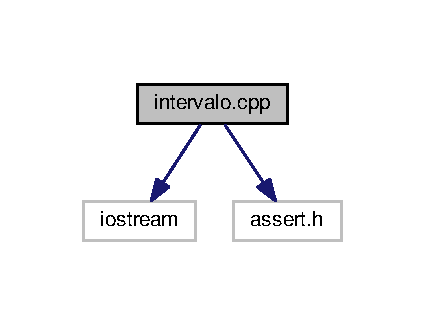
\includegraphics[width=204pt]{intervalo_8cpp__incl}
\end{center}
\end{figure}
\subsection*{Clases}
\begin{DoxyCompactItemize}
\item 
class \hyperlink{classIntervalo}{Intervalo}
\end{DoxyCompactItemize}
\subsection*{Funciones}
\begin{DoxyCompactItemize}
\item 
void \hyperlink{intervalo_8cpp_ae93092259c95b463d176a768b9884802}{escribir} (const \hyperlink{classIntervalo}{Intervalo} \&i)
\begin{DoxyCompactList}\small\item\em Imprime los valores de un intervalo de forma visual según lo indicado en el guión. \end{DoxyCompactList}\item 
void \hyperlink{intervalo_8cpp_a81ca561257a3eea794e139a64fdd6593}{leer} (\hyperlink{classIntervalo}{Intervalo} \&i)
\begin{DoxyCompactList}\small\item\em Lee los valores del intervalo según el formato indicado en el guión. \end{DoxyCompactList}\item 
int {\bfseries main} ()\hypertarget{intervalo_8cpp_ae66f6b31b5ad750f1fe042a706a4e3d4}{}\label{intervalo_8cpp_ae66f6b31b5ad750f1fe042a706a4e3d4}

\end{DoxyCompactItemize}


\subsection{Descripción detallada}
\begin{DoxyAuthor}{Autor}
decsai.\+ugr.\+es 
\end{DoxyAuthor}


\subsection{Documentación de las funciones}
\index{intervalo.\+cpp@{intervalo.\+cpp}!escribir@{escribir}}
\index{escribir@{escribir}!intervalo.\+cpp@{intervalo.\+cpp}}
\subsubsection[{\texorpdfstring{escribir(const Intervalo \&i)}{escribir(const Intervalo &i)}}]{\setlength{\rightskip}{0pt plus 5cm}void escribir (
\begin{DoxyParamCaption}
\item[{const {\bf Intervalo} \&}]{i}
\end{DoxyParamCaption}
)}\hypertarget{intervalo_8cpp_ae93092259c95b463d176a768b9884802}{}\label{intervalo_8cpp_ae93092259c95b463d176a768b9884802}


Imprime los valores de un intervalo de forma visual según lo indicado en el guión. 


\begin{DoxyParams}{Parámetros}
{\em i} & El intervalo \\
\hline
\end{DoxyParams}
\index{intervalo.\+cpp@{intervalo.\+cpp}!leer@{leer}}
\index{leer@{leer}!intervalo.\+cpp@{intervalo.\+cpp}}
\subsubsection[{\texorpdfstring{leer(\+Intervalo \&i)}{leer(Intervalo &i)}}]{\setlength{\rightskip}{0pt plus 5cm}void leer (
\begin{DoxyParamCaption}
\item[{{\bf Intervalo} \&}]{i}
\end{DoxyParamCaption}
)}\hypertarget{intervalo_8cpp_a81ca561257a3eea794e139a64fdd6593}{}\label{intervalo_8cpp_a81ca561257a3eea794e139a64fdd6593}


Lee los valores del intervalo según el formato indicado en el guión. 


\begin{DoxyParams}{Parámetros}
{\em i} & El intervalo \\
\hline
\end{DoxyParams}

%--- End generated contents ---

% Index
\backmatter
\newpage
\phantomsection
\clearemptydoublepage
\addcontentsline{toc}{chapter}{Índice}
\printindex

\end{document}
